%----------------------------------------------------------------------
\myframe{Maturity of the Fields of HPO and NAS}{
	\myit{
		\item \alert{Hyperparameter optimization is quite mature}
		\myit{
			\item[-] Blackbox HPO has been researched for decades; \\ there are many software packages
			\item[-] Multi-fidelity HPO has become somewhat mature
			\item[-] Gradient-based HPO is still a nascent field
		}
\medskip
\pause
		\item \alert{Neural architecture search is still a very young field}
		\myit{
			\item[-] It \emph{can} improve results
			\item[-] But rarely in the first trial; failure modes with terrible performance
			\item[-] Blackbox \& multi-fidelity NAS somewhat mature, but slow
		}
\medskip
\pause
		\item \alert{HPO is crucial for good performance; NAS is a bonus}
		\myit{
			\item[-] You \alert{need} to tune your hyperparameters (learning rate, etc)
			\item[-] NAS is not wide-spread yet, for lack of reliable approaches \& software
		}
	}
}
%----------------------------------------------------------------------

%----------------------------------------------------------------------
\myframe{Case Study: NAS \& HPO in Auto-DispNet}{
	\begin{columns}[T]
		\column{0.64\textwidth}
		\myit{
			\item Problem: disparity estimation
			\myit{
				\item[-] Estimate depth from stereo images
			}
	\onslide<2->{
	\bigskip
				\item Background: U-Net
			\myit{
				\item Skip connections from similar spatial resolution to avoid loosing information
			}
	}\onslide<3->{
	\bigskip
				\item Search space for DARTS
			\myit{
				\item 3 cells: keeping spatial resolution, downsampling, 
				and \alert{new upsampling cell that supports U-Net like skip connections} 
			}
		}
		}
		\column{0.35\textwidth}
		\centering
		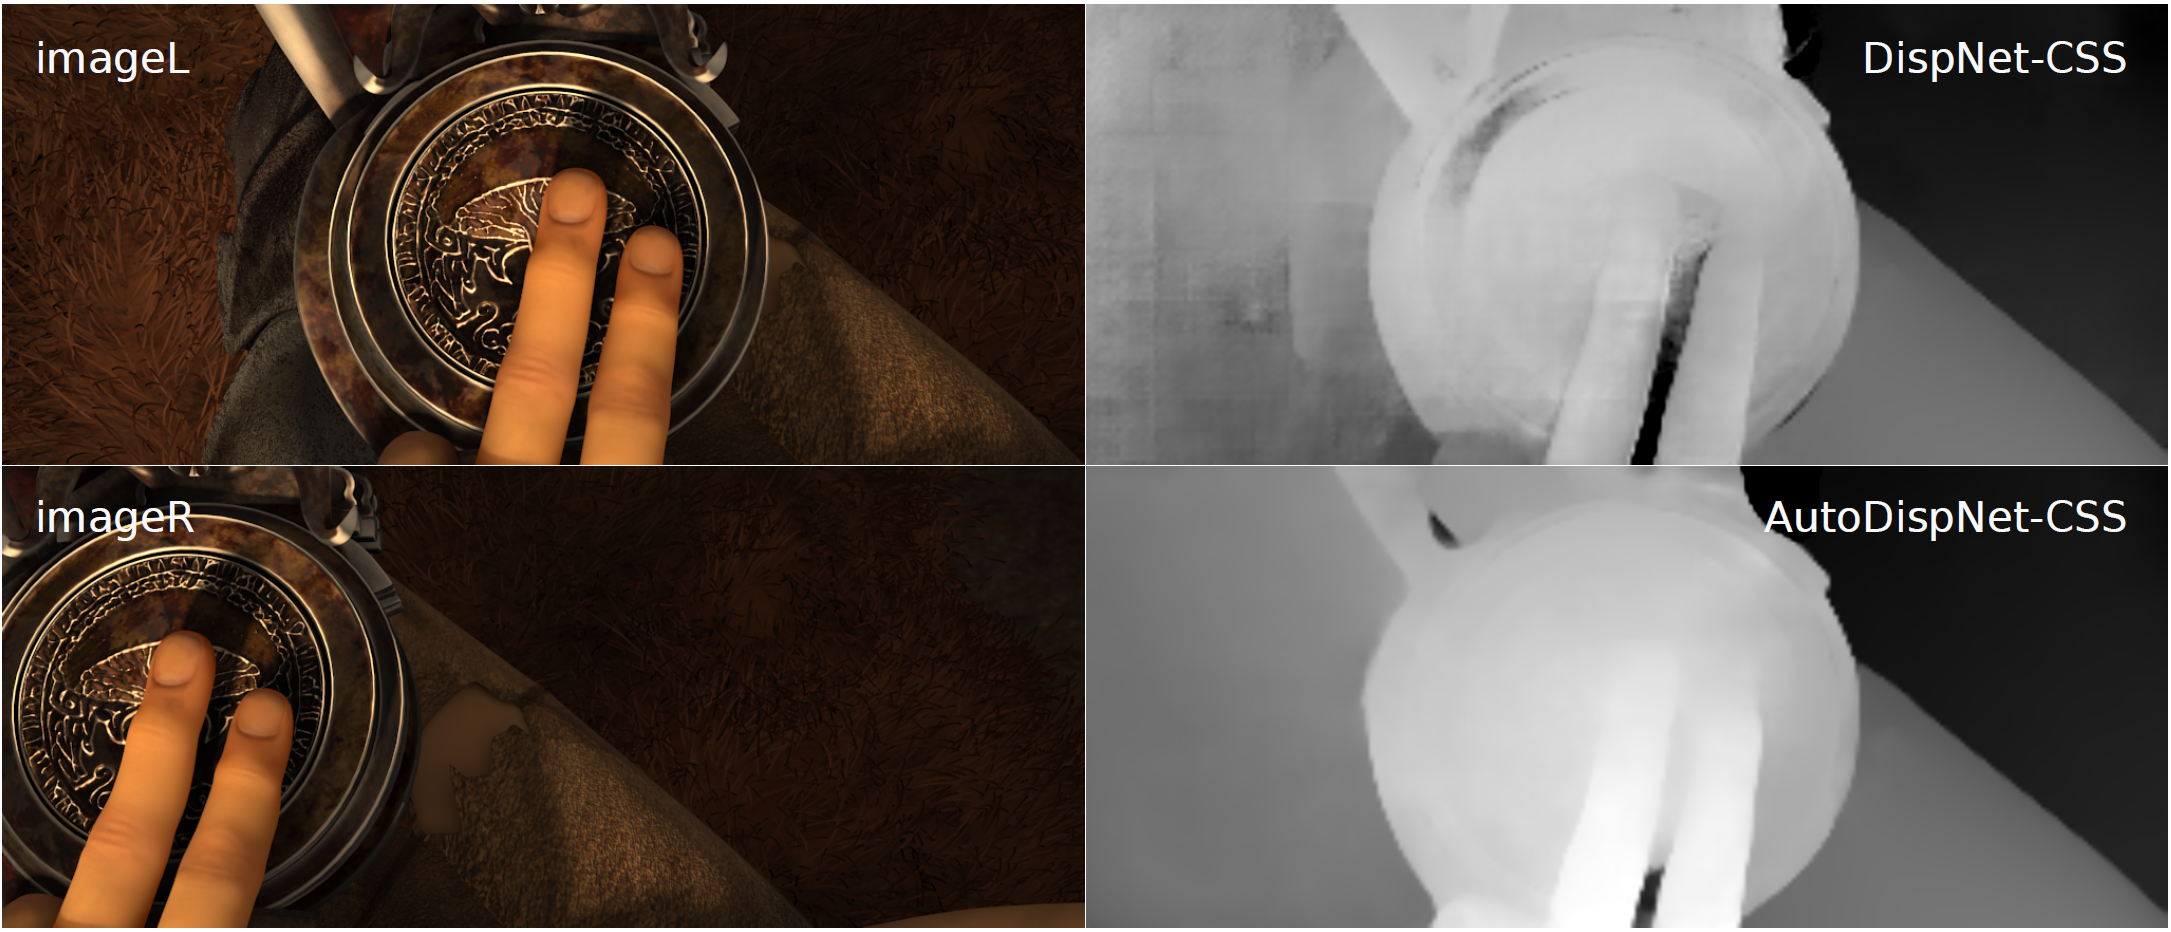
\includegraphics[width=\linewidth]{images/disparity_estimation}\\
\bigskip
\bigskip
\onslide<2->
		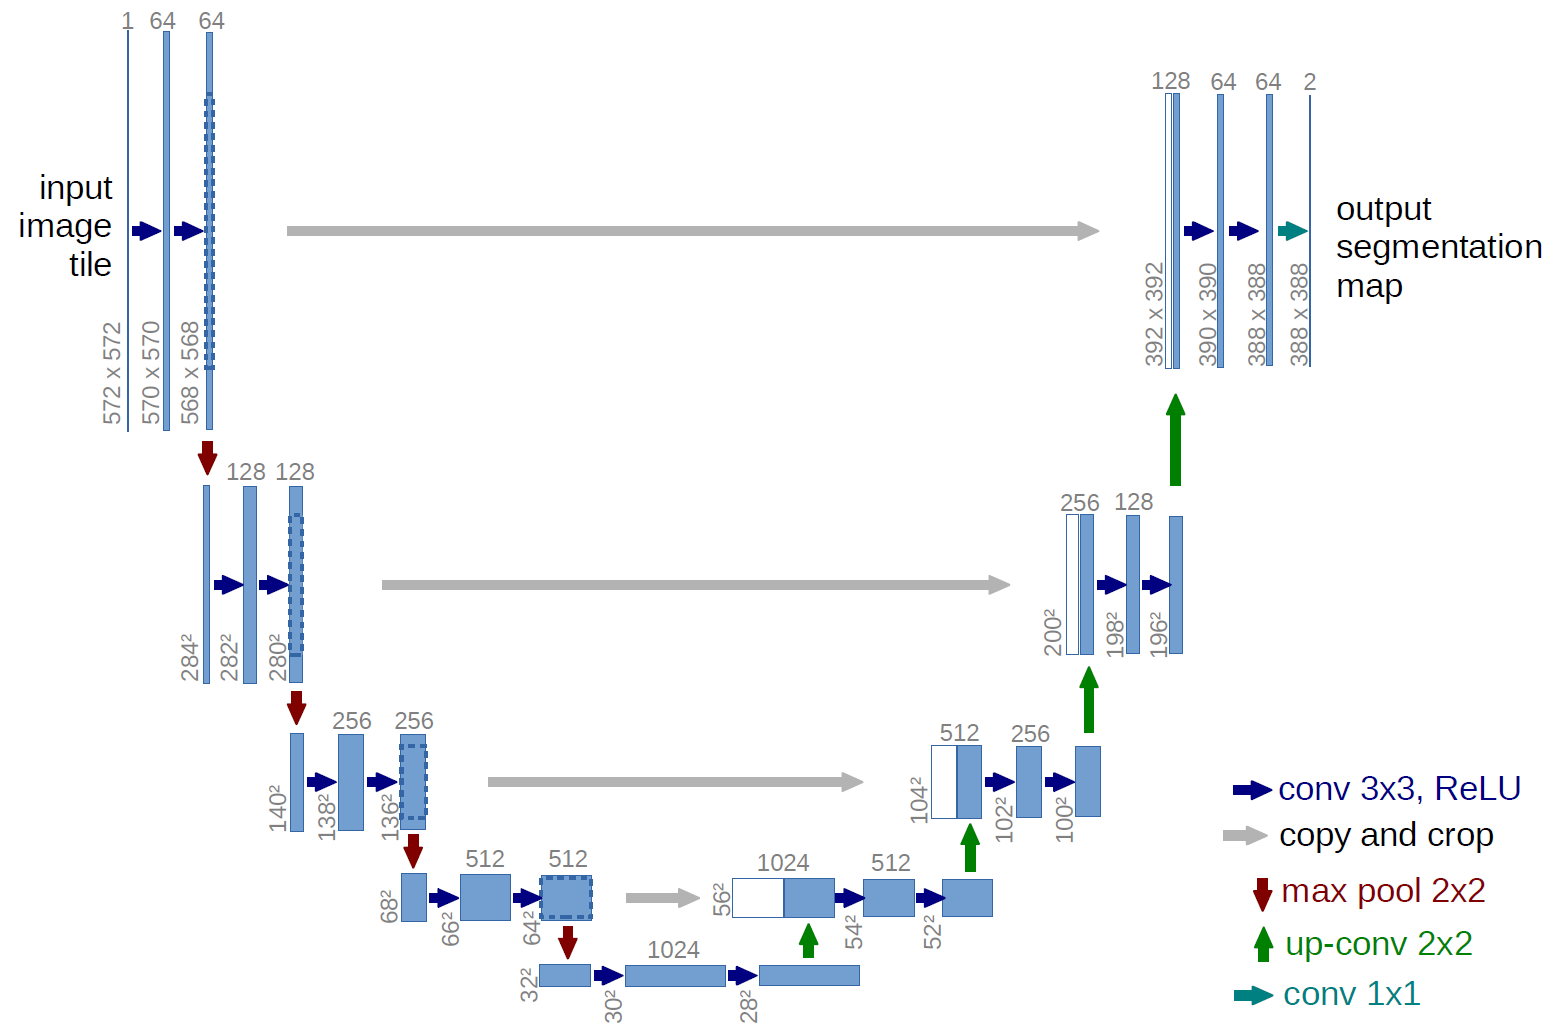
\includegraphics[width=\linewidth]{images/u-net-architecture}	 
	\end{columns}	

	\bigskip
	\bigskip
	\onslide<4->{
		\myit{
			\item Both NAS and HPO improved the state of the art \lit{\href{https://arxiv.org/abs/1905.07443}{Saikat et al, 2019}}:
			\myit{
				\item End-point-error (EPE) on Sintel dataset: \alert{2.36 $\rightarrow$ 2.14 (by DARTS)}
				\item Subsequent HPO: \alert{2.14 $\rightarrow$ 1.94 (by BOHB)}
			}
		}
	}
}
%----------------------------------------------------------------------

%----------------------------------------------------------------------
\myframe{Case Study Details (Auto-DispNet)}{
	\myit{
		\item Very important: \alert{warmstarting} of the network weights
		\myit{
			\item First half of the training epochs: \\
			keep one-shot architecture weights fixed to the uniform distribution
			\item Only afterwards: \\
			DARTS' alternating updates of weights and architectural parameters
		}
\bigskip
		\item Without warmstarting:\\
		\alert{DARTS found cells with only parameterless operations}
	}	
}
%----------------------------------------------------------------------

%----------------------------------------------------------------------
\myframe{Failure Modes of DARTS}{
	\begin{columns}
		\column{0.5\textwidth}
\vspace*{-0.5cm}
		\myit{
			\item Identified 12 small search spaces where DARTS fails badly\\ \lit{Zela et al, 2019}
			\item In all 12 cases, \alert{DARTS only selected parameterless operations, such as skip connections} 
	\medskip
	\medskip
	\medskip
\onslide<2->{
			\item Overfitting of validation loss
			\item Can be fixed by more regularization:\\$L_2$ (for the inner objective), droppath, or early stopping
		}
		}
		\column{0.5\textwidth}	
		\begin{center}
\vspace*{-0.2cm}
		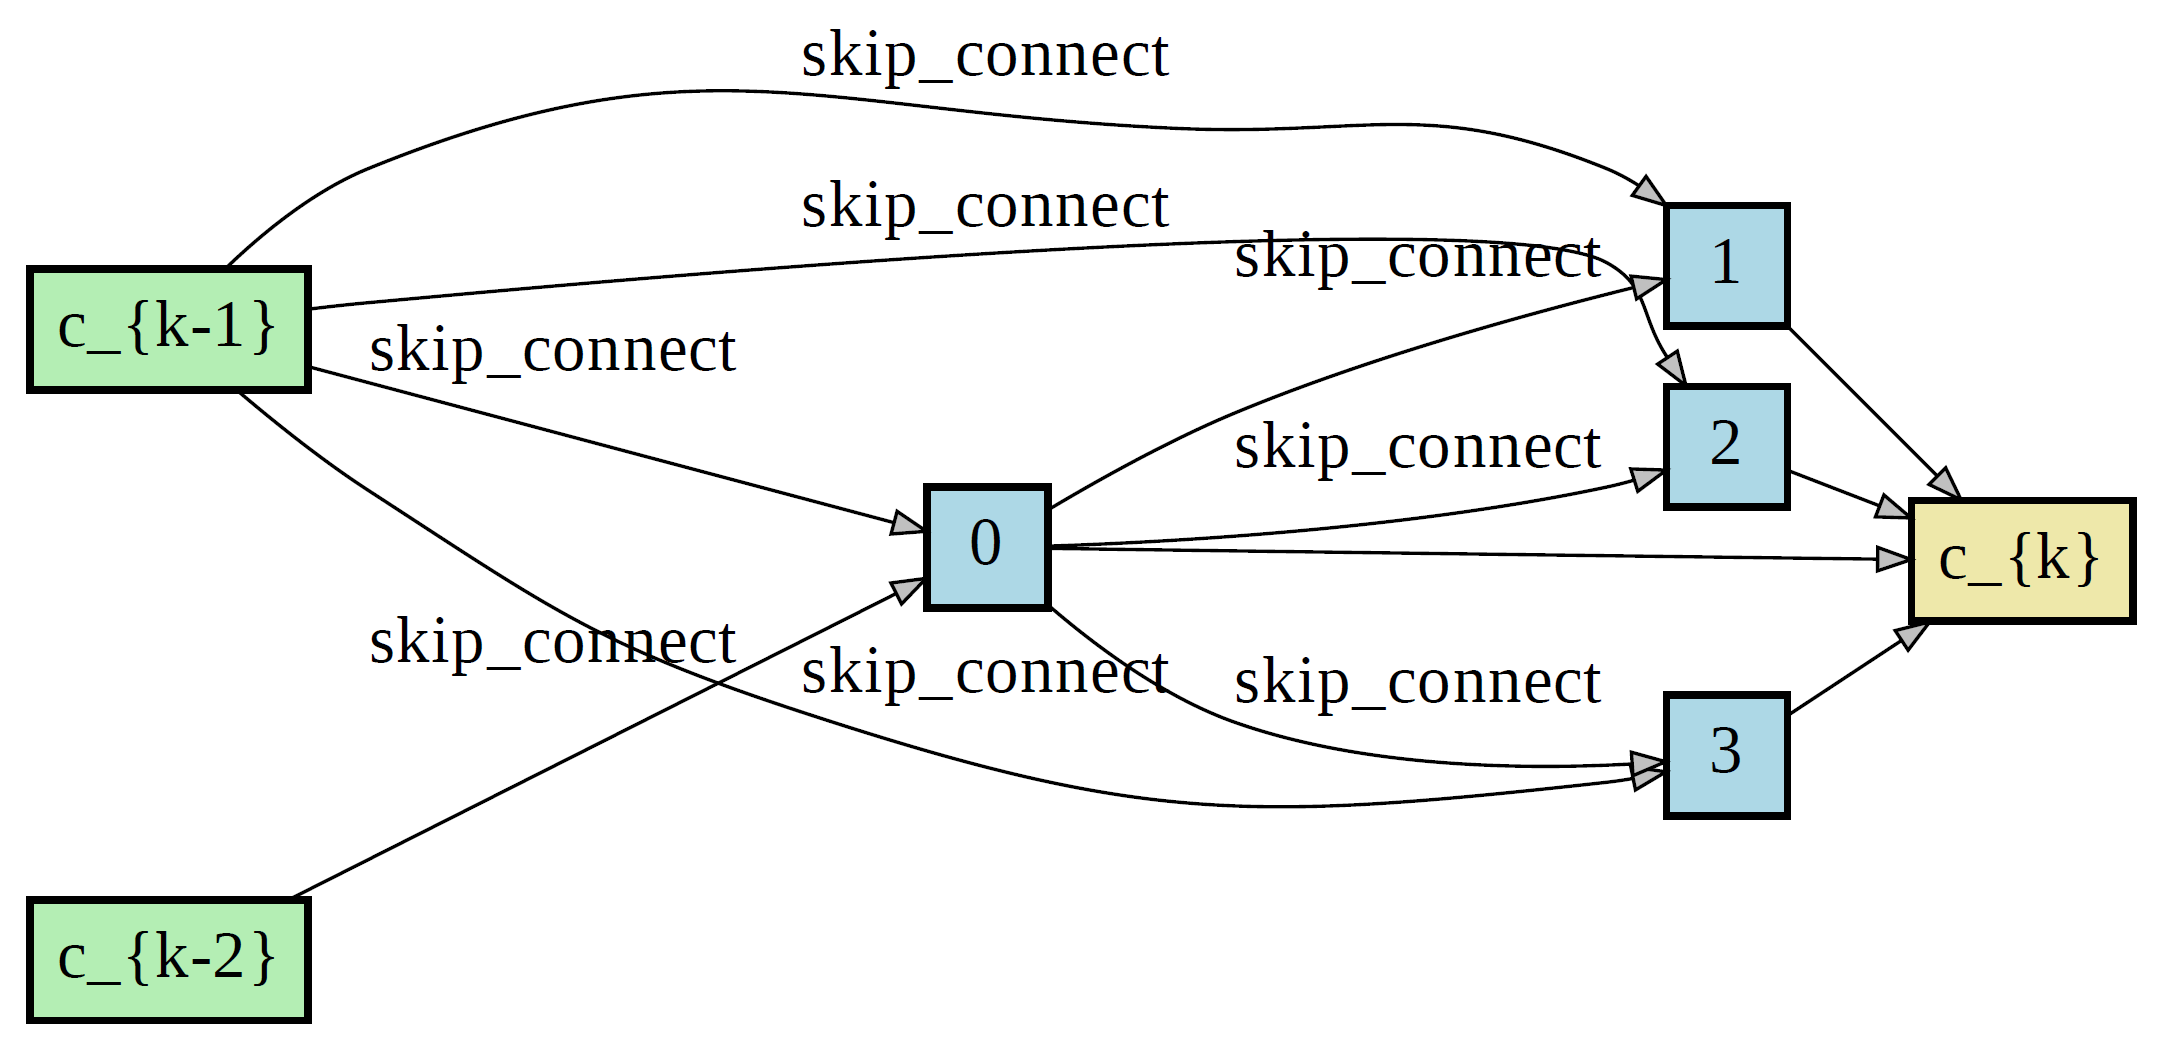
\includegraphics[width=0.9\linewidth]{images/DARTS_example_skip_connects}\\~\\
\vspace*{0.3cm}
\onslide<2->{
		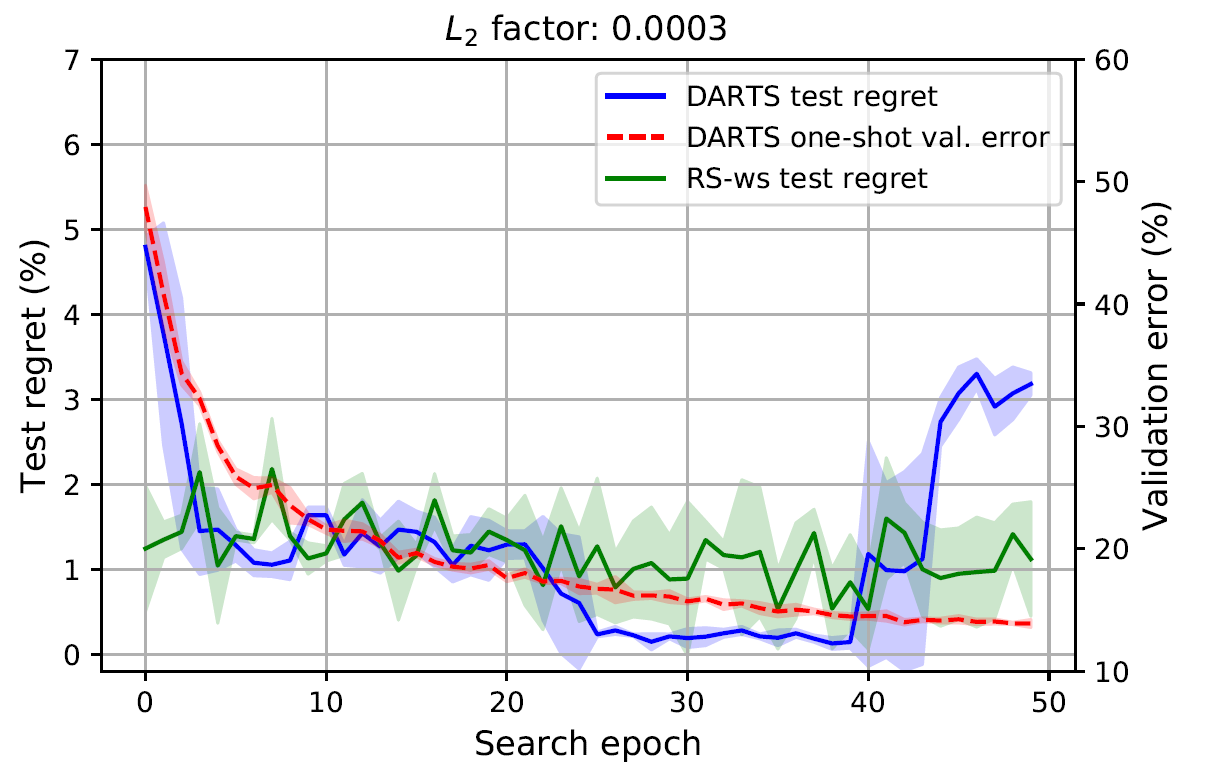
\includegraphics[width=0.9\linewidth]{images/DARTS_overfitting}
}
		\end{center}
	\end{columns}
}
%----------------------------------------------------------------------

%----------------------------------------------------------------------
\myframe{Recommendations for NAS and HPO}{
	\myit{
		\item HPO (in particular: BOHB) typically works; NAS works sometimes
		\myit{
			\item[$\rightarrow$] Always run HPO
			\item[$\rightarrow$] Try NAS if you can 
		}
\bigskip
\pause
		\item How to combine NAS \& HPO
		\myit{
			\item[-] If the compute budget suffices, optimize them jointly using BOHB
			\myit{
				\item[+] Auto-Net / Auto-PyTorch \lit{\href{http://proceedings.mlr.press/v64/mendoza_towards_2016.html}{Mendoza et al, 2016}}
				\item[+] Auto-RL \lit{\href{https://arxiv.org/abs/1812.11951}{Runge et al, 2019}}
			}
\medskip
\pause
			\item[-] \alert{If you don't have decent hyperparameters: first run HPO}	
			\item[-] If you have decent hyperparameters:\\
			run NAS, followed by HPO for fine-tuning \lit{\href{https://arxiv.org/abs/1905.07443}{Saikat et al, 2019}}
\medskip
\pause
			\item[-] To improve robustness of DARTS, \\
			tune DARTS' own hyperparameters with BOHB \lit{\href{https://openreview.net/forum?id=SJx9ngStPH}{Zela et al, 2020}}
		}
	}
}
%----------------------------------------------------------------------

%----------------------------------------------------------------------
\myframe{Questions to Answer for Yourself / Discuss with Friends}{

	\myit{
		\item Repetition:\\ \alert{Describe a failure mode of DARTS. How can it be avoided?}
%\medskip
%		\item Repetition:\\ \alert{When should you apply HPO, when NAS?}
\medskip
		\item Discussion:\\ \alert{If you wanted to use HPO and NAS for your problems,\\ which approach would you use?}
	}	 
}
%-----------------------------------------------------------------------

%----------------------------------------------------------------------
%\myframe{Learning Goals}{
%
%	After this week's videos on HPO and NAS, you should be able to \ldots
%	
%	\begin{itemize}
%		\item describe \alert{several ways of speeding up over blackbox NAS}  %(except via meta-learning)
%		\item describe \alert{several ways of speeding up over blackbox NAS}  %(except via meta-learning)
%		\myit{
%			\item define \alert{network morphisms} \& \alert{explain how to use them to speed up NAS}
%			\item explain various \alert{multi-fidelity Bayesian optimization methods}
%		}
%		\item discuss \alert{when and how to use NAS and HPO in practice} 
%		\item describe \alert{failure modes of DARTS}
%	\end{itemize}
%}

